\documentclass{article}\usepackage[]{graphicx}\usepackage[]{color}
%% maxwidth is the original width if it is less than linewidth
%% otherwise use linewidth (to make sure the graphics do not exceed the margin)
\makeatletter
\def\maxwidth{ %
  \ifdim\Gin@nat@width>\linewidth
    \linewidth
  \else
    \Gin@nat@width
  \fi
}
\makeatother

\definecolor{fgcolor}{rgb}{0.345, 0.345, 0.345}
\newcommand{\hlnum}[1]{\textcolor[rgb]{0.686,0.059,0.569}{#1}}%
\newcommand{\hlstr}[1]{\textcolor[rgb]{0.192,0.494,0.8}{#1}}%
\newcommand{\hlcom}[1]{\textcolor[rgb]{0.678,0.584,0.686}{\textit{#1}}}%
\newcommand{\hlopt}[1]{\textcolor[rgb]{0,0,0}{#1}}%
\newcommand{\hlstd}[1]{\textcolor[rgb]{0.345,0.345,0.345}{#1}}%
\newcommand{\hlkwa}[1]{\textcolor[rgb]{0.161,0.373,0.58}{\textbf{#1}}}%
\newcommand{\hlkwb}[1]{\textcolor[rgb]{0.69,0.353,0.396}{#1}}%
\newcommand{\hlkwc}[1]{\textcolor[rgb]{0.333,0.667,0.333}{#1}}%
\newcommand{\hlkwd}[1]{\textcolor[rgb]{0.737,0.353,0.396}{\textbf{#1}}}%

\usepackage{framed}
\makeatletter
\newenvironment{kframe}{%
 \def\at@end@of@kframe{}%
 \ifinner\ifhmode%
  \def\at@end@of@kframe{\end{minipage}}%
  \begin{minipage}{\columnwidth}%
 \fi\fi%
 \def\FrameCommand##1{\hskip\@totalleftmargin \hskip-\fboxsep
 \colorbox{shadecolor}{##1}\hskip-\fboxsep
     % There is no \\@totalrightmargin, so:
     \hskip-\linewidth \hskip-\@totalleftmargin \hskip\columnwidth}%
 \MakeFramed {\advance\hsize-\width
   \@totalleftmargin\z@ \linewidth\hsize
   \@setminipage}}%
 {\par\unskip\endMakeFramed%
 \at@end@of@kframe}
\makeatother

\definecolor{shadecolor}{rgb}{.97, .97, .97}
\definecolor{messagecolor}{rgb}{0, 0, 0}
\definecolor{warningcolor}{rgb}{1, 0, 1}
\definecolor{errorcolor}{rgb}{1, 0, 0}
\newenvironment{knitrout}{}{} % an empty environment to be redefined in TeX

\usepackage{alltt}
\usepackage[utf8]{inputenc}
\usepackage{amsmath}
\usepackage{graphicx}
%\usepackage{bbold}
\usepackage{tikz}
%\usepackage{silence}
\usepackage{mdframed}
%\WarningFilter{mdframed}{You got a bad break}
\usepackage[colorinlistoftodos]{todonotes}
%\usepackage{listings}
\usepackage{listingsutf8}
\usepackage{color}
\colorlet{exampcol}{blue!10}
\usepackage{multicol}
\usepackage[answerdelayed]{exercise}
\usepackage{booktabs}
\usepackage{caption}

\title{BIO311: Population Ecology\\ \textit{Prac 9: Population Matrices \& LTRE}}

\setcounter{tocdepth}{1} % Determines the depth of the table of contents;; 0:chapters, 1: chapters and sections, 2: chapters,sections and subsections

%\renewcommand{\theExercise}{\thechapter.\arabic{Exercise}}%
\IfFileExists{upquote.sty}{\usepackage{upquote}}{}
\begin{document}

\author{Timoth\'ee Bonnet \&\footnote{This document was co-authored by Tina Cornioley}\; Koen van Benthem\\\\
\tt{timothee.bonnet@ieu.uzh.ch}\\ \tt{koen.vanbenthem@ieu.uzh.ch}}

\date{Spring 2016}





\maketitle
\tableofcontents
\vspace{3cm}
\newpage

%%%%%%%%%%%%%%%%%%%%%%%%%%%%%%%%%%%%%%%%%%%%
%%%%%%%%%%%%%%%% LTREs %%%%%%%%%%%%%%%%%%%%%
%%%%%%%%%%%%%%%%%%%%%%%%%%%%%%%%%%%%%%%%%%%%
\section{Life Table Response Experiment}
Life table response experiments (LTREs) are used to assess which  differences in vital rates lead to a change in $\lambda$ in an experimental design. The experiment you performed on the rotifers is well suited to be analysed by an LTRE. More information on the LTREs can be find in Caswell (2001) \textit{Matrix population models}, this is also the book that we based the theoretical background of this practical on. Before analysing the rotifer data, we will first perform a simple LTRE analysis on different data. During this part of the practical, we will write some of the functions that we will use later to analyse the rotifer data. In practical 6 (last tuesday) we had a short introduction on functions. We repeat (and slightly extend) it here, to refresh your memory.
\begin{mdframed}
\textbf{Functions} so far we have worked with variables that represent a value or set of values, for example \texttt{rot} is a variable that we have defined that contains our data. A function is in a sense a variable that does not contain values, but instead contains a set of tasks. When you call a variable, \texttt{R} will show the value of that variable. When you call a function, \texttt{R} will perform the set of tasks in that function. In general when you want to define a function, it will look like this:
\begin{knitrout}
\definecolor{shadecolor}{rgb}{0.969, 0.969, 0.969}\color{fgcolor}\begin{kframe}
\begin{alltt}
name_of_new_function <- \hlkwd{function}(input_1,input_2,...)\{

  do stuff
  
  \hlkwd{return}(output)
\}
\end{alltt}
\end{kframe}
\end{knitrout}
Let's try to make that less abstract with an example:
\begin{knitrout}
\definecolor{shadecolor}{rgb}{0.969, 0.969, 0.969}\color{fgcolor}\begin{kframe}
\begin{alltt}
\hlstd{x_sq} \hlkwb{<-} \hlkwa{function}\hlstd{(}\hlkwc{x}\hlstd{)\{}
  \hlkwd{return}\hlstd{(x}\hlopt{^}\hlnum{2}\hlstd{)}
\hlstd{\}}

\hlkwd{x_sq}\hlstd{(}\hlnum{3}\hlstd{)}
\end{alltt}
\begin{verbatim}
## [1] 9
\end{verbatim}
\end{kframe}
\end{knitrout}
Here we have first defined a function (\texttt{x\textunderscore sq}) that takes one input variable (\texttt{x}). This function returns the squared value of the input. We can use the function by typing \texttt{x\textunderscore sq(x)}. The advantage of a function as that we don't have to rewrite the code all the time. If we now want to square a different number, we can just type:
\begin{knitrout}
\definecolor{shadecolor}{rgb}{0.969, 0.969, 0.969}\color{fgcolor}\begin{kframe}
\begin{alltt}
\hlkwd{x_sq}\hlstd{(}\hlnum{5}\hlstd{)}
\end{alltt}
\begin{verbatim}
## [1] 25
\end{verbatim}
\begin{alltt}
\hlkwd{x_sq}\hlstd{(}\hlnum{7}\hlstd{)}
\end{alltt}
\begin{verbatim}
## [1] 49
\end{verbatim}
\end{kframe}
\end{knitrout}
Of course, this is not very usefull when the operation that we perform is just simply squaring a number, but when the operations (or set of operations) become more complicated, functions are a great way to save time.

Similarly we can also make a function that adds up two numbers and returns the squared sum:
\begin{knitrout}
\definecolor{shadecolor}{rgb}{0.969, 0.969, 0.969}\color{fgcolor}\begin{kframe}
\begin{alltt}
\hlstd{x_y_sq} \hlkwb{<-} \hlkwa{function}\hlstd{(}\hlkwc{x}\hlstd{,}\hlkwc{y}\hlstd{)\{}
  \hlstd{ans} \hlkwb{<-} \hlstd{x} \hlopt{+} \hlstd{y}
  \hlkwd{return}\hlstd{(ans}\hlopt{^}\hlnum{2}\hlstd{)}
\hlstd{\}}
\hlkwd{x_y_sq}\hlstd{(}\hlnum{3}\hlstd{,} \hlnum{4}\hlstd{)}
\end{alltt}
\begin{verbatim}
## [1] 49
\end{verbatim}
\end{kframe}
\end{knitrout}
One important thing to realise is that things that happen in a function, usually stay in a function (there are ways around this, but in general it is good practice to keep it that way). This means that the tasks in the function are performed in their own 'world' and as soon as the function is executed, the changes are gone.
\begin{knitrout}
\definecolor{shadecolor}{rgb}{0.969, 0.969, 0.969}\color{fgcolor}\begin{kframe}
\begin{alltt}
\hlstd{x_y_sq} \hlkwb{<-} \hlkwa{function}\hlstd{(}\hlkwc{x}\hlstd{,}\hlkwc{y}\hlstd{)\{}
  \hlstd{ans} \hlkwb{<-} \hlstd{x} \hlopt{+} \hlstd{y}
  \hlkwd{return}\hlstd{(ans}\hlopt{^}\hlnum{2}\hlstd{)}
\hlstd{\}}
\hlkwd{x_y_sq}\hlstd{(}\hlnum{3}\hlstd{,} \hlnum{4}\hlstd{)}
\end{alltt}
\begin{verbatim}
## [1] 49
\end{verbatim}
\begin{alltt}
\hlstd{ans}
\end{alltt}


{\ttfamily\noindent\bfseries\color{errorcolor}{\#\# Error in eval(expr, envir, enclos): object 'ans' not found}}\end{kframe}
\end{knitrout}
We now get an error, because \texttt{ans} only exists in the function and is deleted as soon as the function is completed. 
\begin{knitrout}
\definecolor{shadecolor}{rgb}{0.969, 0.969, 0.969}\color{fgcolor}\begin{kframe}
\begin{alltt}
\hlstd{ans} \hlkwb{<-} \hlnum{4}
\hlstd{x_y_sq} \hlkwb{<-} \hlkwa{function}\hlstd{(}\hlkwc{x}\hlstd{,}\hlkwc{y}\hlstd{)\{}
  \hlstd{ans} \hlkwb{<-} \hlstd{x} \hlopt{+} \hlstd{y}
  \hlkwd{return}\hlstd{(ans}\hlopt{^}\hlnum{2}\hlstd{)}
\hlstd{\}}
\hlkwd{x_y_sq}\hlstd{(}\hlnum{3}\hlstd{,} \hlnum{4}\hlstd{)}
\end{alltt}
\begin{verbatim}
## [1] 49
\end{verbatim}
\end{kframe}
\end{knitrout}
What will now be the value of \texttt{ans}?

We have seen that we can not access the version of \texttt{ans} that 'lives' inside the function anymore, once the function has run. If you change anything in a function, you best return these changes to \texttt{R} at the end of the function using \texttt{return()}. Please note that when a function executes \texttt{return(x)}, \texttt{x} is given back to \texttt{R} and anything that comes after it will not be executed.
\end{mdframed}

We will now write a function that calculates the sensitivities of $\lambda$ to the matrix elements. Writing a general function, will make it easier for us to calculate sensitivities for matrices later (which we will do frequently). We provide two options for doing so: by numerical perturbation as we did in the previous practical, or by using the exact solution. The latter is conceptually more difficult, but more precise and less code. You may choose yourself which one you want to implement. Do try to write your function such that it can handle matrices with different sizes.

\begin{mdframed}\textbf{A: Sensitivities using perturbations}\\
Yesterday we have calculated the sensitivities for a barn owl population. We can now re-use that code and put it in a function, so we can use it to from now on easily calculate sensitivities for new matrices. Below the outline is given.

\begin{knitrout}
\definecolor{shadecolor}{rgb}{0.969, 0.969, 0.969}\color{fgcolor}\begin{kframe}
\begin{alltt}
\hlcom{# We are going to make a function with the name}
\hlcom{# sens, that takes 1 input variable: a matrix. We call this}
\hlcom{# matrix A. Everything between \{ and \} is the code}
\hlcom{# of the function. At the end the function uses return()}
\hlcom{# to give back the calculated values of the sensitivities}
\hlstd{sens} \hlkwb{<-} \hlkwa{function}\hlstd{(}\hlkwc{A}\hlstd{)\{}

  \hlstd{da} \hlkwb{<-} \hlnum{1e-4} \hlcom{# define a small perturbation}
  \hlstd{lam} \hlkwb{<-} \hlstd{...}  \hlcom{# extract the dominant eigenvalue of A}
  \hlstd{dim} \hlkwb{<-} \hlstd{...} \hlcom{# store the size of A. Use ncol()}
             \hlcom{# use ?ncol to see what it does}

  \hlcom{# finally, create an empty matrix to store your results in}
  \hlstd{output} \hlkwb{<-} \hlkwd{matrix}\hlstd{(}\hlnum{0}\hlstd{,}\hlkwc{ncol}\hlstd{=dim,}\hlkwc{nrow}\hlstd{=dim)}

  \hlcom{# loop over all indices [i,j] in A, rows and columns}
  \hlcom{# to calculate the sensitivity of each and every index}
  \hlkwa{for}\hlstd{(i} \hlkwa{in} \hlstd{...)\{}
    \hlkwa{for}\hlstd{(j} \hlkwa{in} \hlstd{...)\{}
      \hlstd{TempA} \hlkwb{<-} \hlstd{A} \hlcom{# we copy the matrix}
      \hlstd{TempA[i,j]} \hlkwb{<-} \hlstd{...} \hlcom{# we perturb one element}
      \hlstd{TemLam} \hlkwb{<-} \hlstd{...} \hlcom{# get lambda of the perturbed matrix}
      \hlstd{output[i,j]} \hlkwb{<-} \hlstd{...} \hlcom{# calculate the sensitivity of }
                         \hlcom{#lambda to a[i,j] (dlambda/da)}
    \hlstd{\}}
  \hlstd{\}}

  \hlcom{# In higher dimensions, some eigenvalues may have complex parts}
  \hlcom{# These are not relevant for the sensitivity analysis }
  \hlcom{# (because the sensitivities will not have complex parts)}
  \hlcom{# we still add the following line to R to make sure that R does}
  \hlcom{# not annoy us constantly by adding a +0i (+ an imaginary part of 0)}
  \hlcom{# to the outcomes}
  \hlstd{output} \hlkwb{<-} \hlkwd{Re}\hlstd{(output)}

  \hlkwd{return}\hlstd{(output)} \hlcom{# The end of the function is reached, }
                 \hlcom{# we now return the value of output}
\hlstd{\}}
\end{alltt}
\end{kframe}
\end{knitrout}
\end{mdframed}

\begin{mdframed}
\textbf{B: Sensitivities using the exact solution}\\
Here we will use the formula that was shown in the lecture:
\begin{equation}
\begin{pmatrix} 
\frac{\partial \lambda}{\partial a_{1,1}} & \frac{\partial \lambda}{\partial a_{1,2}} & \dots & \frac{\partial \lambda}{\partial a_{1,N}} \\ 
\frac{\partial \lambda}{\partial a_{2,1}} & \frac{\partial \lambda}{\partial a_{2,2}} & \dots & \frac{\partial \lambda}{\partial a_{2,N}}\\
\vdots & \vdots & & \vdots \\
\frac{\partial \lambda}{\partial a_{N,1}} & \frac{\partial \lambda}{\partial a_{N,2}} & \dots & \frac{\partial \lambda}{\partial a_{N,N}} \\ 
\end{pmatrix}
=
 \frac{\vec{v} \vec{w}^T}{\vec{v}^T \vec{w}}
\end{equation}
Here, $\vec{w}$ and $\vec{v}$ are the dominant right and left eigenvector respectively. Furthermore $\vec{v}^T$ responds to the transpose of $\vec{v}$ (try \texttt{?t} in \texttt{R}). The product of two vectors can be performed in \texttt{R} by using the \texttt{\%*\%} operator. Using this we can now wite a function to calculate the sensitivities:
\begin{knitrout}
\definecolor{shadecolor}{rgb}{0.969, 0.969, 0.969}\color{fgcolor}\begin{kframe}
\begin{alltt}
\hlstd{sens} \hlkwb{<-} \hlkwa{function}\hlstd{(}\hlkwc{A}\hlstd{)\{}
  \hlstd{w} \hlkwb{<-} \hlstd{...}
  \hlstd{v} \hlkwb{<-} \hlstd{...}
  \hlstd{outcome} \hlkwb{<-} \hlstd{...} \hlopt{/} \hlkwd{as.numeric}\hlstd{(...)}
  \hlcom{# here we have to add the as.numeric argument.}
  \hlcom{# this is just a problem of R:}
  \hlcom{# it sees that the number comes from a vector}
  \hlcom{# multiplication and therefore stores it as a matrix}
  \hlcom{# with dimension 1x1. However, it then has difficulties}
  \hlcom{# to divide a matrix by another matrix. We therefore}
  \hlcom{# explicitly have to tell R that this 1x1 matrix is just}
  \hlcom{# a number.}

  \hlcom{# Next: we delete the imaginary part:}
  \hlstd{outcome} \hlkwb{<-} \hlkwd{Re}\hlstd{(outcome)}
  \hlkwd{return}\hlstd{(outcome)}
\hlstd{\}}
\end{alltt}
\end{kframe}
\end{knitrout}

\end{mdframed}
Now test your function on the following two matrices, to make sure that it works.

\begin{knitrout}
\definecolor{shadecolor}{rgb}{0.969, 0.969, 0.969}\color{fgcolor}\begin{kframe}
\begin{alltt}
\hlstd{A} \hlkwb{<-} \hlkwd{matrix}\hlstd{(}\hlkwd{c}\hlstd{(}\hlnum{0.5}\hlstd{,}\hlnum{0.3}\hlstd{,}\hlnum{0.75}\hlstd{,}\hlnum{0.9}\hlstd{),}\hlkwc{nrow}\hlstd{=}\hlnum{2}\hlstd{)}
\hlkwd{sens}\hlstd{(A)}
\end{alltt}
\begin{verbatim}
##           [,1]      [,2]
## [1,] 0.3057428 0.2913858
## [2,] 0.7284644 0.6942572
\end{verbatim}
\begin{alltt}
\hlstd{B} \hlkwb{<-} \hlkwd{matrix}\hlstd{(}\hlkwd{c}\hlstd{(}\hlnum{0.5}\hlstd{,}\hlnum{0.3}\hlstd{,}\hlnum{0.7}\hlstd{,}\hlnum{0.9}\hlstd{,}\hlnum{0.3}\hlstd{,}\hlnum{0.2}\hlstd{,}\hlnum{0.4}\hlstd{,}\hlnum{0.8}\hlstd{,}\hlnum{0}\hlstd{),}\hlkwc{nrow}\hlstd{=}\hlnum{3}\hlstd{)}
\hlkwd{sens}\hlstd{(B)}
\end{alltt}
\begin{verbatim}
##           [,1]      [,2]      [,3]
## [1,] 0.4497062 0.3238265 0.2729042
## [2,] 0.4412927 0.3177681 0.2677985
## [3,] 0.3831683 0.2759136 0.2325257
\end{verbatim}
\end{kframe}
\end{knitrout}
This is a very good start! We now have a function that easily provides us with the sensitivity values for any matrix. From here, we can finally think about more biological problems!
\subsection{Comparison of two populations of mice}
We will now continue with the more biological part of the practical and examine two populations of yellow-necked mice. 

\begin{figure}[h]
\centering
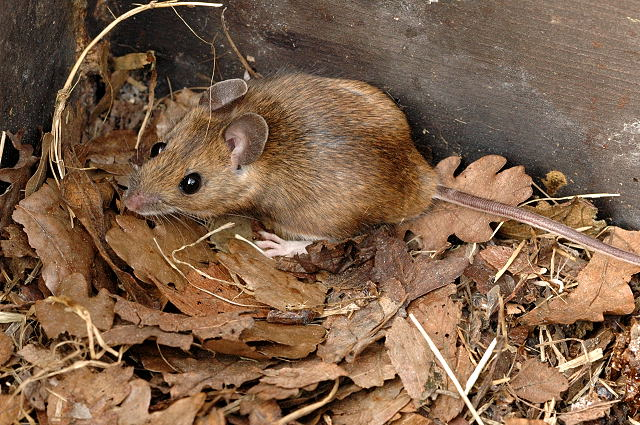
\includegraphics[width=0.3\textwidth]{mouse.jpg}
\caption{\label{fig:mice}yellow-necked mouse, from wikipedia.}
\end{figure}

This species lives mostly in woodlands and it is suspected that its distribution is limited by altitude. Let us compare a population living in the mountain (population $\boldsymbol{M}$) with a population living in the plain (population $\boldsymbol{P}$) to see if the altitude is a limiting distribution factor. This species can be described by a life-cylce in two stages; juveniles and adults. Thus the matrices describing those populations are given by:

\begin{equation}
\boldsymbol{P}=\begin{pmatrix}
0&2\\
0.25&0.5
\end{pmatrix}
\end{equation}
and
\begin{equation}
\boldsymbol{M}=\begin{pmatrix}
0&1.9\\
0.2&0.45
\end{pmatrix}
\end{equation}
Find the asymptotic growth rates of these populations. You can see that they differ. We would now like to investigate which matrix elements contribute the most to the difference in the asymptotic growth rates between the two populations. As before, we will start by looking at the sensitivities: which parameter seems to have the biggest effect on $\lambda$?

The sensitivites give us an idea of what might happen in the future. It shows how much $\lambda$ would increase if a matrix elemant increases with a certain amount. For this, we look at the equations. As we have shown before:
\begin{equation}
s_{i,j} = \frac{\partial \lambda}{\partial a_{i,j}}
\end{equation}
from this it also follows that:
\begin{equation}
s_{i,j} \partial a_{i,j} = \partial \lambda
\end{equation}
So what we see is that if a matrix element increases with an amount of $\partial a_{i,j}$, $\lambda$ will increase with an amount of $\partial \lambda$. For our population however, we know how big the difference in $a_{i,j}$ are from looking at the differences between the matrices (for example, there is a difference of 0.25-0.2=\ensuremath{-0.05} in the maturation rate between the two populations). If we want to know how much each of these differences contributes to differences in $\lambda$, all we have to do with these differences is multiply them with the sensitivities of the corresponding elements.

There is one problem however, which sensitivities do we take? The ones from $\boldsymbol{M}$ or the ones from $\boldsymbol{P}$? In practice what we do is that we use the sensitivities of the average matrix, to make sure that our sensitivities are not biased towards one of the two matrices. 

Using these values, we can describe the asymptotic growth rate of the mountain population matrix, $\boldsymbol{M}$, as a function of the asymptotic growth rate of the plain population matrix, $\boldsymbol{P}$ , our reference population plus a treatment effect:  
\begin{equation}\label{a}
\lambda^{(M)} \approx \lambda^{(P)}+\sum_{i,j}{(a^{(M)}_{ij}-a^{(P)}_{ij})} \frac{ \partial\lambda^{A}}{\partial a^{A}_{ij}}
\end{equation}
Below we explain the different terms:
\begin{itemize}
\item $\lambda^{(P)}$ is the asymptotic growth rate of the $\boldsymbol{P}$ matrix. 
\item The term ${(a^{(M)}_{ij}-a^{(P)}_{ij})}$, is the change in the elements of the matrix due to the treatment effect, here the moutain habitat. It tells us how different an element in matrix $\boldsymbol{M}$ is from the element at the same position in matrix $\boldsymbol{P}$.
\item The last part, $\frac{ \partial\lambda^{A}}{\partial a^{A}_{ij}}$, is the sensitivities of the asymptotic growth rate of a "mid-way" matrix to elements of that "mid-way" matrix. This matrix is the mean between $\boldsymbol{P}$ and $\boldsymbol{M}$ and is thus given by 
\begin{equation}
\boldsymbol{A}=\frac{\boldsymbol{M}+\boldsymbol{P}}{2}
\end{equation}
The matrix $\boldsymbol{A}$ is used because we need a matrix to compare matrices $\boldsymbol{P}$ and $\boldsymbol{M}$ against. It is possible to use either matrix $\boldsymbol{P}$ or $\boldsymbol{M}$ instead but this would give more weight to the selected matrix. Therefore we use the matrix that lies just in between.
\item The multiplication of the sensitivities with the summation term defines how much the change in each elements of the matrix due to the treatment affects the asymptotic growth rate. In other word they are the contributions of the $a_{ij}$ to the effect of the habitat on the growth. It is necessary to do this because for example, a large difference between the elements in the same position may in fact have little effect on the growth if the senstitivity for this position is low. 
\end{itemize}

You may have recognized that equation \ref{a} is a linear equation ($y=b+ax$). This method makes the assumption that the relationship between the matrices is linear and that the slope of this equation is given by $\frac{ \partial\lambda^{A}}{\partial a^{A}_{ij}}$.


With equation \ref{a}, find the value of $\lambda^{(\boldsymbol{M})}$ using \texttt{R} and compare it to the value you found earlier. How different are they? More interestingly: which difference in the matrix elements is mainly responsible for this difference? Is it the juvenile survival, the adult survival or the reproductive rate?\\[1.5ex]

\textit{Hint} Find the "mid-way" matrix. For the sensitivities.

\section{Rotifer data analysis}
In this section, you will apply a factorial LTRE to the rotifer data to compare the layers "peak", "pollution" and "recovery". The second factor is the copper treatment with the levels "low", "high", "medium".

\subsection{Rate estimation}
Before we can start with the analysis of the population matrices, we first need... the matrices and thus the rates (survival and reproduction). Here, we have only two stages: juveniles and adults, so we consider a $2\times 2$ matrix. First, we load in the data (we have now uploaded a new data file on OLAT that does not containt the errors that we introduced for the previous labsession):
\begin{knitrout}
\definecolor{shadecolor}{rgb}{0.969, 0.969, 0.969}\color{fgcolor}\begin{kframe}
\begin{alltt}
\hlstd{Rot} \hlkwb{<-} \hlkwd{read.csv}\hlstd{(}\hlstr{"rotifer_data.csv"}\hlstd{)}
\end{alltt}
\end{kframe}
\end{knitrout}
Next, we use the function \texttt{reshape()} to change the format of the data. This will later make it easier to calculate the rates. Make sure that you understand how this function changes the data!
\begin{knitrout}
\definecolor{shadecolor}{rgb}{0.969, 0.969, 0.969}\color{fgcolor}\begin{kframe}
\begin{alltt}
\hlstd{Roti}\hlkwb{<-}\hlkwd{reshape}\hlstd{(Rot,}\hlkwc{timevar}\hlstd{=}\hlstr{"Day"}\hlstd{,}\hlkwc{idvar}\hlstd{=}\hlkwd{c}\hlstd{(}\hlstr{"Clone"}\hlstd{,}\hlstr{"Copper"}\hlstd{,}\hlstr{"Layer"}\hlstd{),}\hlkwc{direction}\hlstd{=}\hlstr{"wide"}\hlstd{)}
\end{alltt}
\end{kframe}
\end{knitrout}
We will now continue and calculte the rates, for this, we first create a new data frame to store the rates in. This data frame is basically 
\begin{knitrout}
\definecolor{shadecolor}{rgb}{0.969, 0.969, 0.969}\color{fgcolor}\begin{kframe}
\begin{alltt}
\hlstd{Rates} \hlkwb{<-} \hlstd{Roti[,}\hlnum{1}\hlopt{:}\hlnum{3}\hlstd{]}
\end{alltt}
\end{kframe}
\end{knitrout}
Before we start, draw a 2 stage life cycle for the rotifers, this will make it easier to keep track of what is happening. We shall now first calculate the adult survival rate for the period from day $1$ to day $2$. We start by looking at adult survival. We assume that we counted all dead individuals. Now, the survival rate can easily be calculated, it should be the number of alive adults on the first day, minus the number of dead adults observed on the second day, divided by the number of alive adults in the first time step.
\begin{knitrout}
\definecolor{shadecolor}{rgb}{0.969, 0.969, 0.969}\color{fgcolor}\begin{kframe}
\begin{alltt}
\hlstd{Rates}\hlopt{$}\hlstd{Sa1} \hlkwb{<-} \hlstd{(Roti}\hlopt{$}\hlstd{Live_Adult.1} \hlopt{-} \hlstd{Roti}\hlopt{$}\hlstd{Dead_Adult.2)}\hlopt{/} \hlstd{Roti}\hlopt{$}\hlstd{Live_Adult.1}
\end{alltt}
\end{kframe}
\end{knitrout}
Next, we look at the maturation rate. We have already calcuated how many adults survived from day 1, to day 2. The total number of adults on day 2 will however be higher than this number. The additional adults should have arrived due to maturation of juveniles. Calculate the maturation rates (the following expression is incomplete):
\begin{knitrout}
\definecolor{shadecolor}{rgb}{0.969, 0.969, 0.969}\color{fgcolor}\begin{kframe}
\begin{alltt}
\hlstd{Rates}\hlopt{$}\hlstd{M1} \hlkwb{<-} \hlstd{(Roti}\hlopt{$}\hlstd{Live_Adult.2} \hlopt{-} \hlstd{....)} \hlopt{/} \hlstd{...}
\end{alltt}
\end{kframe}
\end{knitrout}

When we look into the calculated maturation rates, we will see that it is sometimes higher than 1. The reason is that we have uncertainty in our count data, maybe an adult too many was counted on day 2, or maybe a juvenile too few on day 1. An alternative explanation is that we assume only 1 transition to take place, it is however theoretically possible that within 1 day a juvenile is born and already grows up to the adult stage. Since we have only very few entries that display such problems, we will cut off the maturation rate at 1: we know that it should not be higher than 1. Uncertainty in the data should not change that theoretical assumption.
\begin{knitrout}
\definecolor{shadecolor}{rgb}{0.969, 0.969, 0.969}\color{fgcolor}\begin{kframe}
\begin{alltt}
\hlstd{Rates}\hlopt{$}\hlstd{M1[Rates}\hlopt{$}\hlstd{M1} \hlopt{>} \hlnum{1}\hlstd{]} \hlkwb{<-} \hlnum{1}
\end{alltt}
\end{kframe}
\end{knitrout}
The next rate is the probability for a juvenile to survive but stay a juvenile. Alive juveniles at day 1 that did not mature and that were not observed dead on day 2, should have survived and stayed in the same stage:
\begin{knitrout}
\definecolor{shadecolor}{rgb}{0.969, 0.969, 0.969}\color{fgcolor}\begin{kframe}
\begin{alltt}
\hlstd{Rates}\hlopt{$}\hlstd{Sj1} \hlkwb{<-} \hlstd{(Roti}\hlopt{$}\hlstd{Live_Juv.1} \hlopt{-} \hlstd{...} \hlopt{-} \hlstd{...)}\hlopt{/}\hlstd{...}
\end{alltt}
\end{kframe}
\end{knitrout}
This time we see a few cases were survival is found to be negative. We account for it by setting these rate (again there are not many cases) to zero.

\begin{knitrout}
\definecolor{shadecolor}{rgb}{0.969, 0.969, 0.969}\color{fgcolor}\begin{kframe}
\begin{alltt}
\hlstd{Rates}\hlopt{$}\hlstd{Sj1[Rates}\hlopt{$}\hlstd{Sj1} \hlopt{<} \hlnum{0}\hlstd{]} \hlkwb{<-} \hlnum{0}
\end{alltt}
\end{kframe}
\end{knitrout}
Finally we arrive at the last rate: fecundity. Any juveniles observed on day 2, that are not surviving juveniles from day 1, must be new offspring. Calculate the fecundity rates from this concept:
\begin{knitrout}
\definecolor{shadecolor}{rgb}{0.969, 0.969, 0.969}\color{fgcolor}\begin{kframe}
\begin{alltt}
\hlstd{Rates}\hlopt{$}\hlstd{R1} \hlkwb{<-} \hlstd{...}
\end{alltt}
\end{kframe}
\end{knitrout}
Fortunately, for these rates, no weird values are found. Now continue and calculate the rates for the transition from day 2 to day 3. Check for every rate if some illogical values are calculated and correct them before continuing with the calculation of the next rate.
\begin{knitrout}
\definecolor{shadecolor}{rgb}{0.969, 0.969, 0.969}\color{fgcolor}\begin{kframe}
\begin{alltt}
\hlstd{Rates}\hlopt{$}\hlstd{Sa2} \hlkwb{<-} \hlstd{...}
\hlstd{Rates}\hlopt{$}\hlstd{M2} \hlkwb{<-} \hlstd{...}
\hlstd{Rates}\hlopt{$}\hlstd{Sj2} \hlkwb{<-} \hlstd{...}
\hlstd{Rates}\hlopt{$}\hlstd{R2} \hlkwb{<-} \hlstd{...}
\end{alltt}
\end{kframe}
\end{knitrout}
\begin{knitrout}
\definecolor{shadecolor}{rgb}{0.969, 0.969, 0.969}\color{fgcolor}\begin{kframe}
\begin{alltt}
\hlstd{Rates}\hlopt{$}\hlstd{R1} \hlkwb{<-} \hlstd{(Roti}\hlopt{$}\hlstd{Live_Juv.2} \hlopt{-} \hlstd{Roti}\hlopt{$}\hlstd{Live_Juv.1}\hlopt{*}\hlstd{Rates}\hlopt{$}\hlstd{Sj1)} \hlopt{/} \hlstd{Roti}\hlopt{$}\hlstd{Live_Adult.1}

\hlcom{# 2 --> 3}
\hlstd{Rates}\hlopt{$}\hlstd{Sa2} \hlkwb{<-} \hlstd{(Roti}\hlopt{$}\hlstd{Live_Adult.2} \hlopt{-} \hlstd{Roti}\hlopt{$}\hlstd{Dead_Adult.3)}\hlopt{/} \hlstd{Roti}\hlopt{$}\hlstd{Live_Adult.2}
\hlstd{Rates}\hlopt{$}\hlstd{M2} \hlkwb{<-} \hlstd{(Roti}\hlopt{$}\hlstd{Live_Adult.3} \hlopt{+} \hlstd{Roti}\hlopt{$}\hlstd{Dead_Adult.3} \hlopt{-} \hlstd{Roti}\hlopt{$}\hlstd{Live_Adult.2)} \hlopt{/} \hlstd{Roti}\hlopt{$}\hlstd{Live_Juv.2}
\hlstd{Rates}\hlopt{$}\hlstd{M2[Rates}\hlopt{$}\hlstd{M2} \hlopt{>} \hlnum{1}\hlstd{]} \hlkwb{<-} \hlnum{1}
\hlstd{Rates}\hlopt{$}\hlstd{Sj2} \hlkwb{<-} \hlstd{(Roti}\hlopt{$}\hlstd{Live_Juv.2} \hlopt{-} \hlstd{Roti}\hlopt{$}\hlstd{Dead_Juv.3} \hlopt{-} \hlstd{Roti}\hlopt{$}\hlstd{Live_Juv.2}\hlopt{*}\hlstd{Rates}\hlopt{$}\hlstd{M2)} \hlopt{/} \hlstd{Roti}\hlopt{$}\hlstd{Live_Juv.2}
\hlstd{Rates}\hlopt{$}\hlstd{Sj2[Rates}\hlopt{$}\hlstd{Sj2} \hlopt{<} \hlnum{0}\hlstd{]} \hlkwb{<-} \hlnum{0}
\hlstd{Rates}\hlopt{$}\hlstd{R2} \hlkwb{<-} \hlstd{(Roti}\hlopt{$}\hlstd{Live_Juv.3} \hlopt{-} \hlstd{Roti}\hlopt{$}\hlstd{Live_Juv.2}\hlopt{*}\hlstd{Rates}\hlopt{$}\hlstd{Sj2)} \hlopt{/} \hlstd{Roti}\hlopt{$}\hlstd{Live_Adult.2}
\hlstd{Rates}\hlopt{$}\hlstd{R2[Rates}\hlopt{$}\hlstd{R2} \hlopt{<} \hlnum{0}\hlstd{]} \hlkwb{<-} \hlnum{0}
\end{alltt}
\end{kframe}
\end{knitrout}
We can now plot what these rates look like. For this it is easiest to first reshape the rates. The following two commands allow you to generate a boxplot of the rates for the transition of day 1 to day 2:
\begin{knitrout}
\definecolor{shadecolor}{rgb}{0.969, 0.969, 0.969}\color{fgcolor}\begin{kframe}
\begin{alltt}
\hlkwd{library}\hlstd{(tidyr)}
\hlstd{Rates_plot} \hlkwb{<-} \hlkwd{gather_}\hlstd{(Rates,}\hlstr{"Rate"}\hlstd{,}\hlstr{"Value"}\hlstd{,}\hlkwd{c}\hlstd{(}\hlstr{"Sj1"}\hlstd{,}\hlstr{"Sa1"}\hlstd{,}\hlstr{"M1"}\hlstd{,}\hlstr{"R1"}\hlstd{))}
\hlkwd{boxplot}\hlstd{(Value}\hlopt{~}\hlstd{Copper}\hlopt{+}\hlstd{Rate,Rates_plot)}
\hlkwd{boxplot}\hlstd{(Value}\hlopt{~}\hlstd{Layer}\hlopt{+}\hlstd{Rate,Rates_plot)}
\end{alltt}
\end{kframe}
\end{knitrout}
Here, we use \texttt{gather\_}, try to understand what it does. Then we use \texttt{boxplot}. Here, the first argument specifies what is plotted (in this case the column \texttt{Value} is plotted, but it is split out by the categories \texttt{Copper} and \texttt{Rate} for the first plot. This is parsed to the function by the code \texttt{Value $\sim$ Copper + Rate}, this can be read as: plot the numbers in the column Value, but split them up according to both Copper and Rate). Adapt this code to also plot the rates for the second transition.

Alternatively you may consider using \texttt{ggplot()} to obtain -- depending on your taste -- nicer looking plots.
\begin{knitrout}
\definecolor{shadecolor}{rgb}{0.969, 0.969, 0.969}\color{fgcolor}\begin{kframe}
\begin{alltt}
\hlkwd{library}\hlstd{(ggplot2)}
\hlkwd{ggplot}\hlstd{(Rates_plot,}\hlkwd{aes}\hlstd{(}\hlkwd{factor}\hlstd{(Copper),Value,}\hlkwc{fill}\hlstd{=Rate))} \hlopt{+} \hlkwd{geom_boxplot}\hlstd{()}
\end{alltt}
\end{kframe}
\end{knitrout}
We will now continue and start creating the matrices. For this, first we calculate the average rates for the transition from day 1 to 2 and the one from day 2 to 3. This will allow us to make on matrix and thus one value of $\lambda$ per clone
\begin{knitrout}
\definecolor{shadecolor}{rgb}{0.969, 0.969, 0.969}\color{fgcolor}\begin{kframe}
\begin{alltt}
\hlcom{# Averages}
\hlstd{Rates}\hlopt{$}\hlstd{SaM} \hlkwb{<-} \hlstd{(Rates}\hlopt{$}\hlstd{Sa1} \hlopt{+} \hlstd{Rates}\hlopt{$}\hlstd{Sa2)}\hlopt{/}\hlnum{2}
\hlstd{Rates}\hlopt{$}\hlstd{MM} \hlkwb{<-} \hlstd{...}
\hlstd{Rates}\hlopt{$}\hlstd{SjM} \hlkwb{<-} \hlstd{...}
\hlstd{Rates}\hlopt{$}\hlstd{RM} \hlkwb{<-} \hlstd{...}
\end{alltt}
\end{kframe}
\end{knitrout}

Now we create a new column with the name \texttt{lambda} and using a for-loop, we can now for each replicate calculate the value for lambda, by constructing the appropriate matrix.
\begin{knitrout}
\definecolor{shadecolor}{rgb}{0.969, 0.969, 0.969}\color{fgcolor}\begin{kframe}
\begin{alltt}
\hlstd{Rates}\hlopt{$}\hlstd{lambda} \hlkwb{<-} \hlnum{0} \hlcom{# create empty column}
\hlkwa{for}\hlstd{(i} \hlkwa{in} \hlnum{1}\hlopt{:}\hlkwd{nrow}\hlstd{(Rates))\{} \hlcom{# for each row in Rates}
  \hlstd{Mat} \hlkwb{<-} \hlstd{...}
  \hlstd{Rates}\hlopt{$}\hlstd{lambda[i]} \hlkwb{<-} \hlstd{...}
\hlstd{\}}
\end{alltt}
\end{kframe}
\end{knitrout}
We can now again use the boxplot commands that we used before to see how lambda varies among matrices.
\begin{knitrout}
\definecolor{shadecolor}{rgb}{0.969, 0.969, 0.969}\color{fgcolor}\begin{kframe}
\begin{alltt}
\hlstd{Rates2} \hlkwb{<-} \hlstd{Rates[,}\hlkwd{c}\hlstd{(}\hlstr{'Copper'}\hlstd{,}\hlstr{'Layer'}\hlstd{,}\hlstr{'SaM'}\hlstd{,}\hlstr{'MM'}\hlstd{,}\hlstr{'SjM'}\hlstd{,}\hlstr{'RM'}\hlstd{)]}
\hlstd{Rates3} \hlkwb{<-} \hlkwd{aggregate}\hlstd{( .}\hlopt{~} \hlstd{Copper}\hlopt{+}\hlstd{Layer,Rates2,mean)}
\hlstd{Rates3}\hlopt{$}\hlstd{lambda} \hlkwb{<-} \hlnum{NA}
\hlstd{Rates}\hlopt{$}\hlstd{lambda} \hlkwb{<-} \hlnum{NA}
\hlkwa{for}\hlstd{(i} \hlkwa{in} \hlnum{1}\hlopt{:}\hlkwd{nrow}\hlstd{(Rates3))\{}
  \hlstd{Mat} \hlkwb{<-} \hlkwd{matrix}\hlstd{(}\hlkwd{c}\hlstd{(Rates3}\hlopt{$}\hlstd{SjM[i],Rates3}\hlopt{$}\hlstd{MM[i],Rates3}\hlopt{$}\hlstd{RM[i],Rates3}\hlopt{$}\hlstd{SaM[i]),}\hlkwc{nrow}\hlstd{=}\hlnum{2}\hlstd{)}
  \hlstd{Rates3}\hlopt{$}\hlstd{lambda[i]} \hlkwb{<-} \hlkwd{eigen}\hlstd{(Mat)}\hlopt{$}\hlstd{values[}\hlnum{1}\hlstd{]}
\hlstd{\}}

\hlkwa{for}\hlstd{(i} \hlkwa{in} \hlnum{1}\hlopt{:}\hlkwd{nrow}\hlstd{(Rates))\{}
  \hlstd{Mat} \hlkwb{<-} \hlkwd{matrix}\hlstd{(}\hlkwd{c}\hlstd{(Rates}\hlopt{$}\hlstd{SjM[i],Rates}\hlopt{$}\hlstd{MM[i],Rates}\hlopt{$}\hlstd{RM[i],Rates}\hlopt{$}\hlstd{SaM[i]),}\hlkwc{nrow}\hlstd{=}\hlnum{2}\hlstd{)}
  \hlstd{Rates}\hlopt{$}\hlstd{lambda[i]} \hlkwb{<-} \hlkwd{eigen}\hlstd{(Mat)}\hlopt{$}\hlstd{values[}\hlnum{1}\hlstd{]}
\hlstd{\}}
\hlcom{# boxplot(lambda~Copper+Layer,Rates)}
\end{alltt}
\end{kframe}
\end{knitrout}
\subsection{Factorial LTRE}
\begin{mdframed}
\textbf{Fixed Factorial Designs (Theory)}
Factorial LTRE allows the examination of the effects of several treatments and their interactions. This is the case for your rotifer data where you have a "layer" treatment and a "copper" treatment. We can no longer just compare two treatments with each other, instead we have a whole suite of treatments (9 in total, 3 layers times 3 copper levels). We thus have two factors, both with three levels.

A factorial LTRE is similar to a one-way LTRE; we want to find which differences in matrix elements between a focal matrix and a reference matrix contribute the most to the difference in $\lambda$ between the two matrices. Let us take the matrix "recovery layer and low copper" which we call $\boldsymbol{M}^{r,l}$ as the focal matrix, for this we average the rates over all the replicates that were subject to this treatment ($r,l$). We compare it to the matrix naive to any treatment, which we call $\boldsymbol{M}^{..}$. This matrix is obtained from taking the average rates for all the data. Again we are interested in understanding the effect of the different treatments on the asymptotic growth rates.
\begin{equation}\label{b}
\lambda^{r,l}=\lambda^{..}+\alpha^{r}+\beta^{l}+(\alpha \beta)^{r,l}
\end{equation}
Equation \ref{b} tells us that $\lambda^{r,l}$ can be found from the average matrix (with $\lambda^{..}$) plus an effect from the layer "recovery" ($\alpha^r$), an effect from the copper level "low" ($\beta^l$) and an interaction between the two treatments ($(\alpha \beta)^{r,l}$).

To isolate the effect of each factor, we need to look at them separately. So we examine a matrix $\boldsymbol{M}^{r.}$, where the effect of copper is ignored. The rates of this matrix are calculated as the average of all the matrices with from the layer "recovery". 
\begin{equation}\label{c}
\alpha^{r}=\sum_{ij}(a^{r.}_{ij}-a^{..}_{ij}) \frac{\partial\lambda^{A}}{\partial a^{A}_{ij}}
\end{equation}
The structure of equation \ref{c} is the same as the last part of equation \ref{a}. The matrix $\boldsymbol{A}$ is again a "mid-way" matrix between $\boldsymbol{M}^{r.}$ and $\boldsymbol{M}^{..}$. $\alpha^{r}$ tells us how large the effect of the treatment "layer" is on the asymptotic growth rate. If we want to know which matrix elements are responsible for this effect, we need to look at the separate contributions to $\alpha^r$ ($(a^{r.}_{ij}-a^{..}_{ij}) \frac{\partial\lambda^{A}}{\partial a^{A}_{ij}}$). Analogously we can also calculate the effects for the other layers, e.g. $\alpha^{peak}$.

We do the same for the second factor. We examine a matrix $\boldsymbol{M}^{.l}$, where the effect of the layer is ignored: 
\begin{equation}\label{d}
\beta^{l}=\sum_{ij}(a^{.l}_{ij}-a^{..}_{ij}) \frac{\partial\lambda^{B}}{\partial a^{B}_{ij}}
\end{equation}
For the interaction effect, we apply the same logic. We examine a matrix $\boldsymbol{M}^{rl}$ where both the effects of the layer and the copper level are taken into account so as to capture the effect of the interaction between the two factors. Because we want to isolate the interaction effect, we need to remove the effects of the layer and copper treatment.
\begin{equation}
(\alpha \beta)^{rl}=\sum_{ij}(a^{rl}_{ij}-a^{..}_{ij}) \frac{\partial\lambda^{C}}{\partial a^{C}_{ij}} -\alpha^{r}-\beta^{l}
\end{equation}
So far we have considered only the effect of the layer "recovery" and the copper level "low". Of course this can be extended to all other layers of all treatments. So in general the equations become for the $k^{th}$ level of treatment $1$ and the $m^{th}$ the level of treatment $2$.

\begin{equation}\label{f}
\lambda^{k,m}=\lambda^{..}+\alpha^{k}+\beta^{m}+(\alpha \beta)^{k,m}
\end{equation}
\begin{equation}\label{e}
\alpha^{k}=\sum_{ij}(a^{k.}_{ij}-a^{..}_{ij}) \frac{\partial\lambda^{A}}{\partial a^{A}_{ij}}
\end{equation}
\begin{equation}
\beta^{m}=\sum_{ij}(a^{.m}_{ij}-a^{..}_{ij}) \frac{\partial\lambda^{B}}{\partial a^{B}_{ij}}
\end{equation}
\begin{equation}
(\alpha \beta)^{km}=\sum_{ij}(a^{km}_{ij}-a^{..}_{ij}) \frac{\partial\lambda^{C}}{\partial a^{C}_{ij}} -\alpha^{k}-\beta^{m}
\end{equation}
In these equations:
\begin{align}
A &= \frac{\boldsymbol{M^{k.}} + \boldsymbol{M^{..}}}{2} & B &= \frac{\boldsymbol{M^{.m}} + \boldsymbol{M^{..}}}{2} & C &= \frac{\boldsymbol{M^{km}} + \boldsymbol{M^{..}}}{2}
\end{align}
LTREs provide additional information to the growth rate as it describes how the different treatments affect the growth rate. In particular, LTRE allow a detailed comparison of the effect of a treatment on growth rate by examining the contribution of each survival and fertility rate to the growth rates of populations subjected to different treatment levels.
\end{mdframed}
We are now going to apply this theory on the rotifer data. First write a function that performs an \texttt{LTRE}. That is, if we give it two matrices as input, it calculates the sensitivities of the average matrix (you can call the function \texttt{sens}) and it multiplies this with the difference between the matrices. You don't have to use a loop here, if you use \texttt{A*B}, this is not matrix multiplication, but element wise multiplication between the matrices. To get the first element of the result, it simply multiplies the first matrix entry from A, with the first one from B. For the second element of the results, it multiplies the second from A with the second one from B, this is thus not the same as the matrix multiplication that we have used before!
\begin{knitrout}
\definecolor{shadecolor}{rgb}{0.969, 0.969, 0.969}\color{fgcolor}\begin{kframe}
\begin{alltt}
\hlstd{A} \hlkwb{<-} \hlkwd{matrix}\hlstd{(}\hlkwd{c}\hlstd{(}\hlnum{1}\hlstd{,}\hlnum{2}\hlstd{,}\hlnum{3}\hlstd{,}\hlnum{4}\hlstd{),}\hlkwc{nrow}\hlstd{=}\hlnum{2}\hlstd{)}
\hlstd{B} \hlkwb{<-} \hlkwd{matrix}\hlstd{(}\hlkwd{c}\hlstd{(}\hlnum{1}\hlstd{,}\hlnum{2}\hlstd{,}\hlnum{3}\hlstd{,}\hlnum{4}\hlstd{),}\hlkwc{nrow}\hlstd{=}\hlnum{2}\hlstd{)}
\hlstd{A}
\end{alltt}
\begin{verbatim}
##      [,1] [,2]
## [1,]    1    3
## [2,]    2    4
\end{verbatim}
\begin{alltt}
\hlstd{B}
\end{alltt}
\begin{verbatim}
##      [,1] [,2]
## [1,]    1    3
## [2,]    2    4
\end{verbatim}
\begin{alltt}
\hlstd{A}\hlopt{*}\hlstd{B}
\end{alltt}
\begin{verbatim}
##      [,1] [,2]
## [1,]    1    9
## [2,]    4   16
\end{verbatim}
\end{kframe}
\end{knitrout}

\begin{knitrout}
\definecolor{shadecolor}{rgb}{0.969, 0.969, 0.969}\color{fgcolor}\begin{kframe}
\begin{alltt}
\hlcom{#### FACTORIAL DESIGN LTRE}
\hlstd{LTRE} \hlkwb{<-} \hlkwa{function}\hlstd{(}\hlkwc{A}\hlstd{,}\hlkwc{B}\hlstd{)\{}
  \hlstd{M} \hlkwb{<-} \hlstd{(A}\hlopt{+}\hlstd{B)}\hlopt{/}\hlnum{2}
  \hlstd{(A}\hlopt{-}\hlstd{B)} \hlopt{*} \hlkwd{sens}\hlstd{(M)}
\hlstd{\}}
\end{alltt}
\end{kframe}
\end{knitrout}
Next, we will have to create the mean matrix, to which we will compare all other matrices. Simply take the means of all the rates (\texttt{mean}) and put these rates together in a matrix.
\begin{knitrout}
\definecolor{shadecolor}{rgb}{0.969, 0.969, 0.969}\color{fgcolor}\begin{kframe}
\begin{alltt}
\hlstd{MatMean} \hlkwb{<-} \hlstd{...}
\end{alltt}
\end{kframe}
\end{knitrout}

\begin{knitrout}
\definecolor{shadecolor}{rgb}{0.969, 0.969, 0.969}\color{fgcolor}\begin{kframe}
\begin{alltt}
\hlstd{MatMean} \hlkwb{<-} \hlkwd{matrix}\hlstd{(}\hlkwd{c}\hlstd{(}\hlkwd{mean}\hlstd{(Rates}\hlopt{$}\hlstd{SjM),}\hlkwd{mean}\hlstd{(Rates}\hlopt{$}\hlstd{MM),}\hlkwd{mean}\hlstd{(Rates}\hlopt{$}\hlstd{RM),}\hlkwd{mean}\hlstd{(Rates}\hlopt{$}\hlstd{SaM)),}\hlkwc{nrow}\hlstd{=}\hlnum{2}\hlstd{)}
\end{alltt}
\end{kframe}
\end{knitrout}
Now we proceed and calculate the effect of copper on $\lambda$. For this we have to calculate an average matrix for each copper treatment and compare these with the overall average matrix. To obtain the average matrix, we again use \texttt{aggregate}, but this time we supply a formule: \texttt{.$\sim$Copper}, this means that \texttt{aggregate} will apply the function (in this case we will use \texttt{mean}) on all columns, per coppr level. To make sure that we don't end up with lots of columns, we first take a subset of \texttt{Rates} that only contains the relevant columns.
\begin{knitrout}
\definecolor{shadecolor}{rgb}{0.969, 0.969, 0.969}\color{fgcolor}\begin{kframe}
\begin{alltt}
\hlcom{### Copper treatment}
\hlstd{temp}  \hlkwb{<-} \hlstd{Rates[,}\hlkwd{c}\hlstd{(}\hlstr{'Copper'}\hlstd{,}\hlstr{'SaM'}\hlstd{,}\hlstr{'MM'}\hlstd{,}\hlstr{'SjM'}\hlstd{,}\hlstr{'RM'}\hlstd{)]}
\hlstd{tempc} \hlkwb{<-} \hlkwd{aggregate}\hlstd{(.}\hlopt{~}\hlstd{Copper,temp,mean)}
\end{alltt}
\end{kframe}
\end{knitrout}
Next, we have to build a matrix for each row in \texttt{tempc} and perform an LTRE on each of these matrices compared to the overall mean matrix. To make sure that we can store the result afterwards, we first create an empty list with the right length. Complete the code to obtain the effects of copper through the different matrix elements on $\lambda$.
\begin{knitrout}
\definecolor{shadecolor}{rgb}{0.969, 0.969, 0.969}\color{fgcolor}\begin{kframe}
\begin{alltt}
\hlstd{copper_effect} \hlkwb{<-} \hlkwd{list}\hlstd{(}\hlnum{3}\hlstd{)}
\hlkwa{for}\hlstd{(i} \hlkwa{in} \hlnum{1}\hlopt{:}\hlnum{3}\hlstd{)\{}
  \hlstd{mat} \hlkwb{<-} \hlstd{...}
  \hlstd{copper[[i]]} \hlkwb{<-} \hlstd{...}
\hlstd{\}}
\end{alltt}
\end{kframe}
\end{knitrout}
Finally, we add the names of the copper levels to this list, so we can easily find the right matrix back:
\begin{knitrout}
\definecolor{shadecolor}{rgb}{0.969, 0.969, 0.969}\color{fgcolor}\begin{kframe}
\begin{alltt}
\hlkwd{names}\hlstd{(copper_effect)} \hlkwb{<-} \hlstd{tempc}\hlopt{$}\hlstd{Copper}

\hlcom{# now we can obtain specific copper levels}
\hlcom{# by naming them}
\hlstd{copper_effect[[}\hlstr{'100'}\hlstd{]]}
\end{alltt}
\end{kframe}
\end{knitrout}
What are the total effects of the different copper levels on $\lambda$? Repeat the same procedure for the layer effect.
\begin{knitrout}
\definecolor{shadecolor}{rgb}{0.969, 0.969, 0.969}\color{fgcolor}\begin{kframe}
\begin{alltt}
\hlstd{copper_effect} \hlkwb{<-} \hlkwd{list}\hlstd{(}\hlnum{3}\hlstd{)}
\hlkwa{for}\hlstd{(i} \hlkwa{in} \hlnum{1}\hlopt{:}\hlnum{3}\hlstd{)\{}
  \hlstd{mat} \hlkwb{<-} \hlkwd{matrix}\hlstd{(}\hlkwd{c}\hlstd{(tempc}\hlopt{$}\hlstd{SjM[i],tempc}\hlopt{$}\hlstd{MM[i],tempc}\hlopt{$}\hlstd{RM[i],tempc}\hlopt{$}\hlstd{SaM[i]),}\hlkwc{nrow}\hlstd{=}\hlnum{2}\hlstd{)}
  \hlstd{copper_effect[[i]]} \hlkwb{<-} \hlkwd{LTRE}\hlstd{(mat,MatMean)}
\hlstd{\}}
\hlkwd{names}\hlstd{(copper_effect)} \hlkwb{<-} \hlstd{tempc}\hlopt{$}\hlstd{Copper}

\hlcom{### Layer treatment}
\hlstd{temp}  \hlkwb{<-} \hlstd{Rates[,}\hlkwd{c}\hlstd{(}\hlstr{'Layer'}\hlstd{,}\hlstr{'SaM'}\hlstd{,}\hlstr{'MM'}\hlstd{,}\hlstr{'SjM'}\hlstd{,}\hlstr{'RM'}\hlstd{)]}
\hlstd{templ} \hlkwb{<-} \hlkwd{aggregate}\hlstd{(.}\hlopt{~}\hlstd{Layer,temp,mean)}
\hlstd{layer_effect} \hlkwb{<-} \hlkwd{list}\hlstd{(}\hlnum{3}\hlstd{)}
\hlkwa{for}\hlstd{(i} \hlkwa{in} \hlnum{1}\hlopt{:}\hlnum{3}\hlstd{)\{}
  \hlstd{mat} \hlkwb{<-} \hlkwd{matrix}\hlstd{(}\hlkwd{c}\hlstd{(templ}\hlopt{$}\hlstd{SjM[i],templ}\hlopt{$}\hlstd{MM[i],templ}\hlopt{$}\hlstd{RM[i],templ}\hlopt{$}\hlstd{SaM[i]),}\hlkwc{nrow}\hlstd{=}\hlnum{2}\hlstd{)}
  \hlstd{layer_effect[[i]]} \hlkwb{<-} \hlkwd{LTRE}\hlstd{(mat,MatMean)}
\hlstd{\}}
\hlkwd{names}\hlstd{(layer_effect)} \hlkwb{=} \hlstd{templ}\hlopt{$}\hlstd{Layer}
\end{alltt}
\end{kframe}
\end{knitrout}
Finally, we have to calculate the interactions. Now we can use that we names the lists with the copper and layer effects to efficiently access them. We will have to access these in order to be able to substract the correct fixed effects from each interaction, as described in the theory at the beginning of this section.
\begin{knitrout}
\definecolor{shadecolor}{rgb}{0.969, 0.969, 0.969}\color{fgcolor}\begin{kframe}
\begin{alltt}
\hlstd{temp2}  \hlkwb{<-} \hlstd{Rates[,}\hlkwd{c}\hlstd{(}\hlstr{'Copper'}\hlstd{,}\hlstr{'Layer'}\hlstd{,}\hlstr{'SaM'}\hlstd{,}\hlstr{'MM'}\hlstd{,}\hlstr{'SjM'}\hlstd{,}\hlstr{'RM'}\hlstd{)]}
\hlstd{tempi} \hlkwb{<-} \hlkwd{aggregate}\hlstd{(.}\hlopt{~}\hlstd{Copper}\hlopt{+}\hlstd{Layer,temp2,mean)}
\hlstd{interaction} \hlkwb{<-} \hlkwd{list}\hlstd{(}\hlnum{9}\hlstd{)}
\hlkwa{for}\hlstd{(i} \hlkwa{in} \hlnum{1}\hlopt{:}\hlnum{9}\hlstd{)\{}
  \hlstd{mat} \hlkwb{<-} \hlstd{...}
  \hlstd{interaction[[i]]} \hlkwb{<-} \hlstd{...} \hlopt{-} \hlstd{...}
\hlstd{\}}
\end{alltt}
\end{kframe}
\end{knitrout}
What is left now is to plot the values and to examine the summed effect of each copper level, each layer level and each interaction. One way to plot for example the copper effects is by using \texttt{barplot(matrix(unlist(copper),nrow=4))}. 
\begin{knitrout}
\definecolor{shadecolor}{rgb}{0.969, 0.969, 0.969}\color{fgcolor}\begin{kframe}
\begin{alltt}
\hlcom{### Interactions}
\hlstd{temp2}  \hlkwb{<-} \hlstd{Rates[,}\hlkwd{c}\hlstd{(}\hlstr{'Copper'}\hlstd{,}\hlstr{'Layer'}\hlstd{,}\hlstr{'SaM'}\hlstd{,}\hlstr{'MM'}\hlstd{,}\hlstr{'SjM'}\hlstd{,}\hlstr{'RM'}\hlstd{)]}
\hlstd{tempi} \hlkwb{<-} \hlkwd{aggregate}\hlstd{(.}\hlopt{~}\hlstd{Copper}\hlopt{+}\hlstd{Layer,temp2,mean)}
\hlstd{interaction} \hlkwb{<-} \hlkwd{list}\hlstd{(}\hlnum{9}\hlstd{)}
\hlkwa{for}\hlstd{(i} \hlkwa{in} \hlnum{1}\hlopt{:}\hlnum{9}\hlstd{)\{}
  \hlstd{mat} \hlkwb{<-} \hlkwd{matrix}\hlstd{(}\hlkwd{c}\hlstd{(tempi}\hlopt{$}\hlstd{SjM[i],tempi}\hlopt{$}\hlstd{MM[i],tempi}\hlopt{$}\hlstd{RM[i],tempi}\hlopt{$}\hlstd{SaM[i]),}\hlkwc{nrow}\hlstd{=}\hlnum{2}\hlstd{)}
  \hlstd{interaction[[i]]} \hlkwb{<-} \hlkwd{LTRE}\hlstd{(mat,MatMean)} \hlopt{-} \hlstd{layer_effect[[}\hlkwd{as.character}\hlstd{(tempi}\hlopt{$}\hlstd{Layer[i])]]} \hlopt{-} \hlstd{copper_effect[[}\hlkwd{as.character}\hlstd{(tempi}\hlopt{$}\hlstd{Copper[i])]]}
\hlstd{\}}

\hlcom{### Plots}
\hlkwd{barplot}\hlstd{(}\hlkwd{matrix}\hlstd{(}\hlkwd{unlist}\hlstd{(copper_effect),}\hlkwc{nrow}\hlstd{=}\hlnum{4}\hlstd{),}\hlkwc{beside}\hlstd{=T)}
\end{alltt}
\end{kframe}
\includegraphics[width=\maxwidth]{figure/LAST1-1} 
\begin{kframe}\begin{alltt}
\hlkwd{barplot}\hlstd{(}\hlkwd{matrix}\hlstd{(}\hlkwd{unlist}\hlstd{(layer_effect),}\hlkwc{nrow}\hlstd{=}\hlnum{4}\hlstd{),}\hlkwc{beside}\hlstd{=T)}
\end{alltt}
\end{kframe}
\includegraphics[width=\maxwidth]{figure/LAST1-2} 
\begin{kframe}\begin{alltt}
\hlkwd{barplot}\hlstd{(}\hlkwd{matrix}\hlstd{(}\hlkwd{unlist}\hlstd{(interaction),}\hlkwc{nrow}\hlstd{=}\hlnum{4}\hlstd{),}\hlkwc{beside}\hlstd{=T)}
\end{alltt}
\end{kframe}
\includegraphics[width=\maxwidth]{figure/LAST1-3} 
\begin{kframe}\begin{alltt}
\hlcom{## Summary}
\hlkwd{sapply}\hlstd{(copper_effect,sum)}
\end{alltt}
\begin{verbatim}
##           0          50         100 
##  0.07640375  0.03721408 -0.12917539
\end{verbatim}
\begin{alltt}
\hlkwd{sapply}\hlstd{(layer_effect,sum)}
\end{alltt}
\begin{verbatim}
##        peak        post         rec 
## -0.03549940  0.07093708 -0.03564954
\end{verbatim}
\begin{alltt}
\hlkwd{sapply}\hlstd{(interaction,sum)}
\end{alltt}
\begin{verbatim}
## [1]  0.008626281 -0.004133514 -0.005523681  0.005761845
## [5] -0.002215008  0.005738695 -0.015238295  0.008192686
## [9] -0.003202753
\end{verbatim}
\begin{alltt}
\hlcom{### Outcome check}

\hlstd{Rates3}\hlopt{$}\hlstd{lambda2} \hlkwb{<-} \hlnum{NA}
\hlstd{Rates3}\hlopt{$}\hlstd{lambda3} \hlkwb{<-} \hlnum{NA}
\hlstd{lam_mean} \hlkwb{<-} \hlkwd{lambda}\hlstd{(MatMean)}
\hlkwa{for}\hlstd{(i} \hlkwa{in} \hlnum{1}\hlopt{:}\hlnum{9}\hlstd{)\{}
  \hlstd{Rates3}\hlopt{$}\hlstd{lambda2[i]} \hlkwb{<-} \hlstd{lam_mean} \hlopt{+} \hlkwd{sum}\hlstd{(copper_effect[[}\hlkwd{as.character}\hlstd{(Rates3}\hlopt{$}\hlstd{Copper[i])]])} \hlopt{+}\hlkwd{sum}\hlstd{(layer_effect[[}\hlkwd{as.character}\hlstd{(Rates3}\hlopt{$}\hlstd{Layer[i])]])} \hlopt{+} \hlkwd{sum}\hlstd{(interaction[[i]])}
  \hlstd{Rates3}\hlopt{$}\hlstd{lambda3[i]} \hlkwb{<-} \hlstd{lam_mean} \hlopt{+} \hlkwd{sum}\hlstd{(copper_effect[[}\hlkwd{as.character}\hlstd{(Rates3}\hlopt{$}\hlstd{Copper[i])]])} \hlopt{+}\hlkwd{sum}\hlstd{(layer_effect[[}\hlkwd{as.character}\hlstd{(Rates3}\hlopt{$}\hlstd{Layer[i])]])}
\hlstd{\}}
\hlstd{Rates3}
\end{alltt}
\begin{verbatim}
##   Copper Layer       SaM        MM       SjM        RM
## 1      0  peak 0.9062771 0.5458333 0.3326389 0.7727273
## 2     50  peak 0.8325397 0.3436177 0.5429563 0.9496032
## 3    100  peak 0.6763889 0.3416667 0.3681818 0.9388889
## 4      0  post 0.8332341 0.5541667 0.4180556 1.0975469
## 5     50  post 0.9101852 0.3851852 0.4828704 1.1138889
## 6    100  post 0.8291667 0.3230519 0.5354978 0.8513889
## 7      0   rec 0.8735119 0.5106151 0.4282738 0.7413690
## 8     50   rec 0.8658069 0.3125000 0.6458333 0.8717262
## 9    100   rec 0.8075397 0.1982143 0.6128968 0.7583333
##     lambda  lambda2  lambda3
## 1 1.329420 1.329012 1.320385
## 2 1.277040 1.277062 1.281196
## 3 1.109256 1.109282 1.114806
## 4 1.432687 1.432584 1.426822
## 5 1.385515 1.385417 1.387632
## 6 1.226945 1.226981 1.221243
## 7 1.305197 1.304997 1.320235
## 8 1.289216 1.289238 1.281045
## 9 1.109948 1.111453 1.114656
\end{verbatim}
\end{kframe}
\end{knitrout}

If you manage to go through all the steps describe above, you should now know the asymptotic growth rates ($\lambda$) of your populations, have performed three LTRE analyses on your rotifer data and have plots to include in your report. The interpretation of the results is up to you.


\begin{center}
Good luck!
\end{center}

\begin{figure}[h]
\centering
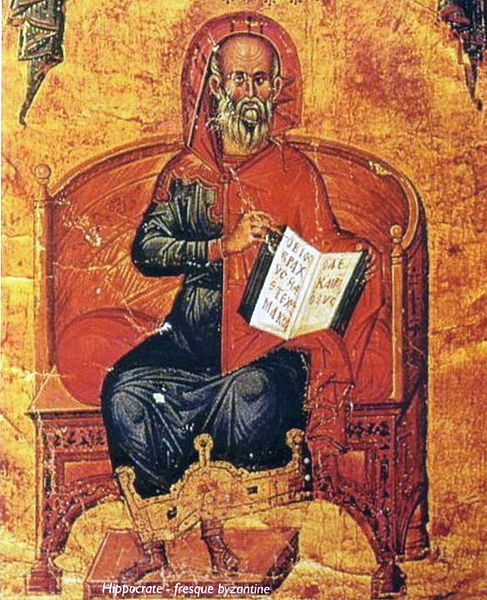
\includegraphics[width=0.3\textwidth]{Hippocrate.jpg}
\caption{\label{fig:owl}random picture, from wikipedia.}
\end{figure}

\end{document}
